\documentclass{article}
\usepackage{amsfonts, amsmath, amssymb, amsthm} % Math notations imported
\usepackage{enumitem}
\usepackage{graphicx}
\usepackage{setspace}
\usepackage{indentfirst}
\usepackage[margin=1in]{geometry}
\graphicspath{{./images/}} % Path to images

% \begin{figure}[htb!]
%      \centering
%      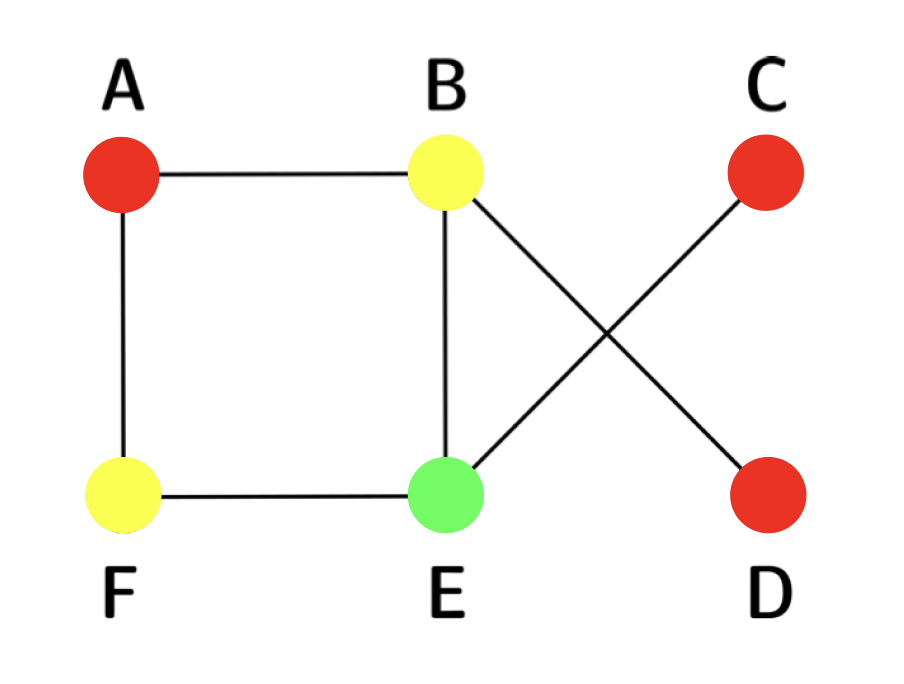
\includegraphics[scale=0.5]{coloring.png}
%      \caption{Coloring of the graph.}
% \end{figure}

\newtheorem{thm}{Theorem}
\newtheorem{proposition}[thm]{Proposition}
\newtheorem{cor}[thm]{Corollary}

% title information
\title{Math 104 HW2}
\author{Neo Lee}
\date{09/08/2023}

\setstretch{1.15}
% main content
\begin{document} 

% placing title information; comment out if using fancyhdr
\maketitle 

\section*{Exercise 4.1}
For each set below that is bounded above, list three upper bounds for the set. Otherwise write 
"NOT BOUNDED ABOVE". 

\textbf{(a)} [0,1]

\textbf{(c)} \{2,7\}

\textbf{(e)} $\{\frac{1}{n}:n\in\mathbb{N}\}$

\textbf{(g)} [0,1] $\cup$ [2,3]

\textbf{(i)} $\cap^\infty_{n=1}\left[\frac{-1}{n}, 1+\frac{1}{n}\right]$

\textbf{(k)} $\{n+\frac{(-1)^n}{n}:n\in\mathbb{N}\}$

\textbf{(m)} $\{r\in\mathbb{Q}:r^2<4\}$

\textbf{(o)} $\{x\in\mathbb{R}:x<0\}$

\textbf{(q)} \{0, 1, 2, 4, 8, 16\}

\textbf{(s)} $\{\frac{1}{n}:n\in\mathbb{N} \emph{ and } n \emph{ is prime}\}$

\textbf{(u)} $\{x^2:x\in\mathbb{R}\}$

\textbf{(w)} $\{sin\left(\frac{n\pi}{3}\right):n\in\mathbb{N}\}$

\section*{Exercise 4.2}
Repeat Exercise 4.1 for lower bounds.

\section*{Exercise 4.8}
Let $S$ and $T$ be nonempty subsets of R with the following property: $s\le t$ for all $s\in S$ and 
$t\in T$.
\begin{enumerate}[label=(\alph*)]
    \item Oberserve that $S$ is bounded above and $T$ is bounded below. 
    \item \begin{proposition}
        Sup $S\le$ inf $T$.
    \end{proposition}
    \item Give an exampe of such sets $S$ and $T$ where $S\cap T$ is nonempty.
    \item Give an example of sets $S$ and $T$ where sup $S=$ inf $T$ and $S\cap T$ is an empty set.
\end{enumerate}

\section*{Exercise 4.14}
Let $A$ and $B$ be nonempty bounded subsets of $\mathbb{R}$, and let $A + B$ be the set of all 
sums $a+b$ where $a\in A$ and $b\in B$.
\begin{enumerate}[label=(\alph*)]
    \item \begin{proposition}
        Sup $(A+B) = $ sup $A$ + sup $B$. Hint: To show sup $A$ + sup $B\le$ sup $(A+B)$, show that 
        for each $b \in B$, sup $(A+B)-b$ is an upper bound for $A$, hence sup $A le$ sup 
        $(A + B) - b$. Then show sup $(A + B)$ - sup $A$ is an upper bound for $B$.
    \end{proposition}
    \item \begin{proposition}
        Inf $(A+B) = $ inf $A$ + inf $B$.
    \end{proposition}
\end{enumerate}

\section*{Exercise 4.16}
\begin{proposition}
    Sup $\{r\in\mathbb{Q}:r<a\} = a$ for each $a\in\mathbb{R}$.
\end{proposition}

\section*{Exercise 5.5}
\begin{proposition}
    Inf $S \le$ sup $S$ for every nonempty subset of $\mathbb{R}$. Consider both bounded and 
    unbounded sets.
\end{proposition}
\end{document}
